\documentclass[12pt, letterpaper]{article}
%packages
\usepackage[english]{babel}
\usepackage[utf8]{inputenc}
\usepackage{fancyhdr}%headers/footers
\usepackage{hyperref}%hyper links
\usepackage{amsmath}%fractions and such
\usepackage{listings}%code listing
\usepackage{graphicx}%iamges
\usepackage{float}% H placement parameter - less floaty floats

%document metadata
\title{First document}
\author{Rastislav Kučera}
\date{June 2018}

%page style defines
\fancypagestyle{MyDefault}{\pagestyle{fancy}\fancyhf{}\cfoot{\thepage}}

\fancypagestyle{MyFirstPage}{\pagestyle{fancy}\fancyhf{}\rhead{Rastislav Kučera}\lhead{Semestral project (2)}}

%newcommand


%document setup
\pagestyle{MyDefault}
\hypersetup{
    colorlinks=true,
    linkcolor=blue,
    filecolor=magenta,      
    urlcolor=cyan,
}
\graphicspath{ {./images/} }%image directory


\begin{document}

\begin{titlepage}\centering
\thispagestyle{MyFirstPage}
%Centering and title
\vspace*{\fill}
\LARGE \textbf{General Representation of Light Sources in Photorealistic Computer Graphics} 
\vspace*{\fill}
\end{titlepage}

\section{Introduction}

The goal of this project was to implement in Java a representation of light sources suitable for 
rendering based on \href{https://en.wikipedia.org/wiki/Monte_Carlo_method}{Monte Carlo} solution approaches to the \href{http://www.cse.chalmers.se/edu/year/2011/course/TDA361/2007/rend_eq.pdf}{rendering equation}.

The rendering equation for monochromatic light can be expressed as
\begin{equation}
L(x, \omega)=L_e(x, \omega)+\int_\Omega{\rho(x, \omega', \omega) L(RT(x, -\omega'), \omega') \cos{\theta'} d\omega'}
\label{eq:rendering}
\end{equation}
where the unknown $L(x, \omega)$ is the radiance (``light intensity'', measured in $W sr^{-1}m^{-2}$) leaving the differential area around the surface point $x$ in a differential angle around the direction $\omega$. The given function $L_e(x, \omega)$ is zero everywhere except for points $x$ at the light sources. The given function $\rho(x, \omega', \omega)$ describes the surface materials, more precisely the scattering of light entering the point $x$ from the direction $\omega'$. $\theta$ is the angle between the surface normal at the point $x$ and the direction $\omega$. $RT(x, \omega)$ is a ray tracing function which returns the nearest surface point (different from $x$) from the point $x$ in the direction $\omega$.

The rendering equation is a Fredholm (recursive) integral equation of the second kind. Approaches to solving the equation can be roughly divided into two categories: direct and simplifying. Simplifying approaches such as radiosity and ray tracing transform the rendering equation into a simpler one. However, this not only disallows simulation of all light phenomena governed by the rendering equation but also imposes constraints on the input scene (geometry, materials, light sources, camera). Direct approaches work with unmodified Eq.~\ref{eq:rendering} and unfold the recursion into a series of nested integrals. Although these series are infinite, an iterative evaluation of the integrals converges to the solution of Eq.~\ref{eq:rendering}.

\section{Rendering Equation and Light Sources}

%The emitted radiance $L_e(x, \omega)$ in Eq.~\ref{eq:rendering} describes all light sources in the scene. 
The assumption of the monochromaticity of light can be obliterated by extending the radiance function with the wavelength $\lambda$ (which ranges in the visible spectrum from ca. 400~nm to ca. 700~nm). The rendering equation then becomes
\begin{gather}
L(x, \lambda, \omega)=L_e(x, \lambda, \omega)+\nonumber\\
\int_{\Lambda}{\int_{\Omega}{\rho(x, \lambda', \omega', \lambda, \omega) L(RT(x, -\omega'), \lambda', \omega') \cos{\theta'} d\omega'} d\lambda'}
\label{eq:rendering_spectral}
\end{gather}

%Emissive Case 
In direct solution methods, light sources are generators of (random) beams which transport the radiance from points on the light sources' surfaces. The function $L_e$ serves as a probability distribution function. Sampling of a single light source involves storing two structures in each \textbf{Beam}: \textbf{SpatialData}  ($x$ and $\omega$) and \textbf{ColorData} ($\lambda$). In order to distribute the total power of the source, the number of generated
beams is updated in the light source from which the beams originated. 
%The sum of all beams' pows is at any moment equal to the intensity of Light source they originate from. Knowing this, we can set all Beam intensity to (SourcePower)/(NumberOfBeams)
%$\dfrac{SourcePower}{NumberOfBeams}$ %this is too tall for line
%and rely on extensive enough sampling of Light source, which  will generate different colors with different weights. 
Thus each light source should implement methods \verb|Beam getNextBeam()| which returns a random beam, and \verb|long getNumberOfBeams()| which returns the number of beams which have been generated by this light source. Besides SpatialData and ColorData, each beam stores a reference to its parent light source. Using Java serialization, light sources can be then added to an arbitrary renderer which supports their type.
%maybe add fun fuct : beams are more Rendering equation element, LS are more MonteCarlo element

%add small comments to Reflective And Transmissive case - involves materials
Therefore, every light source implements the following interface:
\begin{lstlisting}[language=Java]
interface LightSource
extends java.io.Serializable {
	Beam getNextBeam();
	long getNumberOfBeams();
}
\end{lstlisting}

Each beam implements methods of the following abstract class:
\begin{lstlisting}[language=Java]
public Beam {
	public SpatialData sd;
	public LightSource parent;
	public ColorData c;
}
\end{lstlisting}

%the 3. function is Beam getDeterministicBeam(PointToIntersect, wavelength) which returns beam that goes somewhere from parent LS, througth Point PointToIntersect with wavelength or nothing. (maybe modifie beam power value) 

\subsection{Representation of color in beams}

Human eye has 3 types of cones (S,M,L) which are sensitive to different, overlapping parts of visible light spectrum.
%, and are more sensitive to different wavelengths in their corresponding part of light spectrum. 
The perceived color depends not only on the wavelengths hitting the eye, but also on the number of photons (beams) which carry the wavelengths.

The \textbf{RGB color model} represents color as a triplet $[r, g, b]$ which expresses how much red, green, and blue is measured by the eye's cones. This model is very useful in output devices such as monitors or images stored on a disk. It is also frequently used in ray tracing to represent colors of light sources and scattering of light on surfaces (the Phong model). Although our representation of light sources is general enough to accommodate the RGB model in light sources and beams, we are aware of that an $[r, g, b]$ triple is a very poor approximation of the visible spectrum. It is insufficient for rendering effects such as \href{https://en.wikipedia.org/wiki/Refraction}{refraction}, \href{https://en.wikipedia.org/wiki/Fluorescence}{fluorescence} etc. 

%Instead of RGB, I will use in this text Spectral representation of color, using Spectral Power Distribution so aforementioned effects would be more realistic.

\subsubsection{Spectral power distribution}

\textbf{Spectral power distribution} (SPD) is a function which describes how much energy is radiated on each wavelength in the visible spectrum. (A data format with the same name is used by e.g. manufacturers of light bulbs.) In the context of this work, we use SPD as a probability distribution function and require that it be normalized, i.e.  its integral over the whole spectrum be equal to 1. This also simplifies the scaling of the power of a light source with one additional parameter (stored in the light source outside of SPD).

An SPD implements the following interface:
\begin{lstlisting}[language=Java]
interface SpectralPowerDistribution{
	double getNextLambda();
	double getValue(double lambda);
	double[] getFirstAndLastLambda();
}
\end{lstlisting}
where \verb|double getNextLambda()| generates one random sample $\lambda$ from the SPD distribution, \verb|double getValue(double lambda)| returns the function value of the SPD, \verb|getFirstAndLastLambda()| returns the limits of the SPD's  domain.

\begin{figure}[H]%need to find/create normalized SPD picture
\centering 
%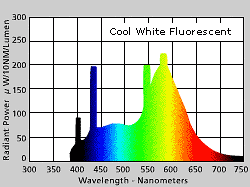
\includegraphics[natwidth=250,natwidth=187]{Spd.png}
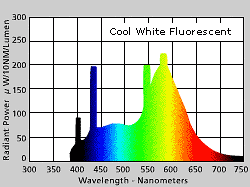
\includegraphics[width=0.6\textwidth]{Spd.png}
\caption{An example of  an (unnormalized) SPD, taken from \href{http://www.lrc.rpi.edu/education/learning/terminology/spectralpowerdistribution.asp}{this website}}
\end{figure}

\subsection{Sampling of wavelengths and beams}

The generation of random beams in SpatialData and random wavelengths in ColorData leads to the problem of discrete samples from a given probability distribution. The number of samples is potentially infinite, but they are generated one by one and their count is kept.

Let us demonstrate the problem on an example.

\begin{figure}[H]
\centering 
%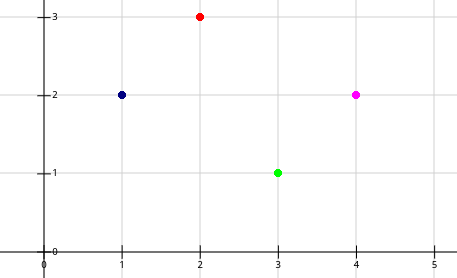
\includegraphics[natwidth=457,natwidth=278]{Samples.png}
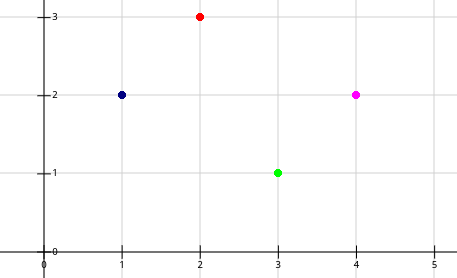
\includegraphics[scale=0.8]{Samples.png}
\caption{Discrete samples taken from a discrete (not necessarily normalized) probability distribution. $X$ is what we want to get, $Y$ is the weight (frequency of appearance) of the desired $X$.}
\end{figure}

In a long run, we want to obtain a sequence with the same amount of 1s and 4s, but only half as many 3s as 1s (or 4s) and three times more 2s than 3s. A simple method to generate such a sequence is to compute the sum $I$ of functional values  from 1 to 4 ($I=8$), then produce a uniform random number $m\in [0,1)$, and then keep summing the functional values for $X$ from 1 to 4 until their sum $S$ is greater than $mI$. The number $X$ which we are after is the last (the largest) X for which $S\le mI$. 
%\textit{I use sum instead of integral, because we do not care about step size in this case.}

The algorithm for sampling an evenly sampled discrete probability distribution is:\\
Input: A discrete probability distribution function $f(X)$ defined on a uniformly spaced set $\{a,...,b\}$.\\
Output: A random sample $X$ from the probability distribution $f(X)$.
\begin{enumerate}
\item Set $I = \sum_{n=a}^{b}f(n)$. Note that  $I=1$ for a ``genuine'' (normalized) probability distribution function $f(X)$.
\item Generate a uniform random number $m\in [0, 1)$.
\item Return the largest $X$ such that $\sum_{n=a}^{X}f(n) \le mI$.
\end{enumerate}

%Problem with this solution is that it creates “Choppy” distribution,what can be suppressed by adding more samples (what would reduce “choppynes”, but increase number of iterations), but not in all  cases, or by replacing gaps with some function that is easy to integrate which would remove “choppynes” completely and make this generator continuous, in which case we have to solve $\int_{a}^{r}h(x) = m*\int_{a}^{b}g(x)$, where $r$ is the result and $h(x)$ is new continuous function composed from $f(x)$ and continuous filler functions $g_n(x)$.

\subsubsection{Linear gap filling functions}

The probability distribution functions we deal with are usually not discrete, although their representations are. For example, consider an SPD which is defined on an interval of visible wavelengths, but is represented by uniformly spaced discrete points in which the function values are known (measured by a spectrometer). When we treat such an SPD as a discrete function, then the distribution of samples generated by the sampling algorithm above will be ``choppy''. 
%The choppiness is reduced when the number of points increases, but this also increases the number of iterations in the last step of the algorithm. 
It is desirable to interpolate the function values between the discrete points. The interpolation can be perceived as an extension of the discrete function $f(X)$ with``gap filling'' functions $g_n(X)$, where the function $g_n(X)$ is defined on the interval  between the successive $n$-th and $(n+1)$-th points of $f(X)$.

%A linear gap filling function on an interval $[A, B]$ is defined as $y - y1 = m*(x-x1)$, where $m = (f(B) - f(A))/(B-A)$ , $y1 = f(A)$, $x1 = A$. This yields
Let a discrete f(X) be defined at points $x_1, \dots, x_N$. A linear gap filling function $g_n(x)$  is then defined on the interval $[x_k, x_{k+1}]$ as
\begin{eqnarray}
g(x) = \frac{f(x_{k+1})-f(x_k)}{x_{k+1}-x_{k}} * (x - x_{k}) + f(x_{k})
\end{eqnarray}

%Let $c_1 = \frac{f(B)-f(A)}{B-A}$ and $c_2 = \frac{f(B)*A+f(A)*B}{B-A}$, then $g_n(x) = c_1*x - c_2$, $x\in [A,B)$ and $\int g_n(x) = c_1\int xdx - c_2\int 1dx = \frac{c_1}{2}x^2 - c_2x =x(\frac{c_1}{2}x - c_2)$.

The following sampling algorithm returns a real random $r$ according to a gap-filled (not necessarily normalized) probability distribution function $f(X)$:
\begin{enumerate}
\item Compute $I = \sum_{i=1}^n {\int_{x_i}^{x_{i+1}} {g_i(x) dx}}$.
\item Generate a uniform random number $m\in [0, 1)$.
%Calculate $i = m*I$, m is random number from $[0,1)$
%\item Find greatest $r_1$ from $\{a,..,b\}$ that sum of integrals for $g_n(x)$ on their respective $[A,B)$ is $< i$
\item Find the largest $j$ such that $\sum_{i=1}^j {\int_{x_i}^{x_{i+1}} g_i(x) dx} \le mI$.
\item Return $r$ from the interval $[x_j, \dots, x_N]$ such that\\ $(\sum_{i=1}^j {\int_{x_i}^{x_{i+1}} g_i(x) dx}) + \int_{x_{j+1}}^r g_{j+1}(x) dx = mI$.
%\item Solve $\int_{r_1}^{r_2}g_n(x) = i - r_1*I$
%\item result is $r = r_1 + r_2$
\end{enumerate}

%In  $\int_{r_1}^{r_2}g_n(x) = i - r_1*I$, the $r_2 = A$ for that $g_n(x)$, so : $r_2(\frac{c_1}{2}r_2-c_2) - A(\frac{c_1}{2}A -c_2) = i - r_1*I$ what is quadratic equation. $D = c_{2}^{2} - 4\frac{c_1}{2}*[A(\frac{c_1}{2}A-c_2)-i+r_1*I]$, so $r_2 = \frac{-c_2 +- \sqrt(D)}{c_1}$.

%\subsubsection{Same amount of wavelengths, but different scales}
%Previously mentioned approach applied in Light source generates different amounts of Beam with different wavelengths (colors).

%Complementary approach would be generating same amounts of all wavelengths(colors), but adding scale/weight value to beams. Scale can be value of lambda on normalized SPD (integral = 1). Power of one Beam would be harder to express.

\section{Examples of concrete light sources}

\subsection{Conventions}

Throughout this section, the following mathematical and physical conventions are used:
\begin{itemize}
\item We work with 3-dimensional Euclidean space. However, points, directions and normals are represented by 4-valued vectors $[x, y, z, w]$, whereby the last value $w$ is implicitly 1 unless stated otherwise.
\item Right-handed cordinate system is used, i.e. $x$ is the horizontal direction (increasing from left to right), $y$ is the vertical direction (increasing from bottom to top), $z$ is the depth (increasing inwards).
\item Transformation matrices are represented by matrices 4x4 \href{https://en.wikipedia.org/wiki/Row-_and_column-major_order}{row major order}.
\item Positive rotations, ordering of vertices  (e.g. of a triangle) etc. are counter-clockwise.
\item Color is represented by SPD. Wavelengths are given in nanometers, not meters.
\end{itemize}

A beam of light (a photon carrying energy from its parent light source on a wavelength $\lambda$) can thus be represented as
\begin{lstlisting}[language=Java]
public class Beam {
	//SpatialData
	public Vector3 origin, direction;
	//LS parent
	public LightSource parent;
	//ColorData
	public double lambda, scale = 1, level = 1;
}
\end{lstlisting}

Note that instead of a using Vector, we could store direction as 2 angles. This would save some memory but would increase the time complexity of computations.

The variable \verb|Beam.scale| represents the weight of a beam, hence the power of the beam is equal to $\frac{Beam.parent.getPower()}{Beam.parent.getNumberOfBeams()} * Beam.scale$. 
%This and \verb|level| variable will be described further in Renderer section. The variable are used when parent light source power is not known (when using less wasteful path creation in bidirectional rendering) and are not needed for simple rendering from Light source.

The class \verb|spdLightSource| is still an abstract class, but it is more concrete than \verb|LightSource| in that it uses SPD to represent the color. The variable \verb|power| is used to scale the intensity of the SPD.
\begin{lstlisting}[language=Java]
public abstract class spdLightSource 
implements LightSource {
	private double power;
	private SpectralPowerDistribution spd;
	private long number_of_beams = 0;
	
	public spdLightSource(
		SpectralPowerDistribution _spd,
		double _power)
	{spd = _spd; power = _power;}
	
	public double getPower()
	{return power;}
}
\end{lstlisting}

The variable \verb|number_of_beams| is increased every time \verb|getNextBeam()| is called. The variable \verb|power| is the total energy released by this light source, hence the energy on a wavelength \verb|lambda| is equal to\\
 \verb|power*spd.getValue(lambda)|.

We are now ready to show the implementation of various concrete light sources. They all are based on the abstract class \verb|spdLightSource|.

\subsection{Laser}

A simple example of a concrete light source is \verb|Laser| which shines from one point in one direction (and often emits light within a very narrow spectrum):
\begin{lstlisting}[language=Java]
public class Laser extends spdLightSource{
	private Vector3 position,direction;	
		
	public Laser(SpectralPowerDistribution _spd, 
	       double _power, Vector3 _position, 
	       Vector3 _direction)
	{
		super(_spd,_power);
		position = _position;
		direction = _direction;		
	}

	public Beam getNextBeam()
	{
		Beam b = new Beam();	
		b.lambda = spd.getNextLambda();
		b.origin = position;
		b.direction = direction;
		number_of_beams++;
		return b;
	}
}
\end{lstlisting}

\subsection{Sky}

The lights source \verb|Sky| is perceived as an infinitely distant rectangular light source covered with \verb|Laser|s radiating light in parallel beams. It
resembles the Sun illuminating the Earth (as the Sun is very far, the beams hitting the Earth are almost parallel).

\begin{lstlisting}[language=Java]
public class Sky extends spdLightSource{
	private Vector3 A, B, direction, 
		fromAverticalDir, 
		fromAhorizontalDir; 
		// A and B are the corners 
		// of the sky rectangle
	private Laser laser;
	private Random verticalr, horizontalr;	
		
	public Sky(SpectralPowerDistribution _spd, 
	       double _power, Vector3 _A, Vector3 _B, 
	       Vector3 _direction)
	{
		. . . initialization . . .
	}

	public Beam getNextBeam()
	{
		Beam b = laser.getNextBeam();
		b.origin += 
		verticalr.getDouble() * 
		fromAverticalDir;
		b.origin += 
		horizontalr.getDouble() * 
		fromAhorizontalDir;
		number_of_beams++;
		return b;
	}
}
\end{lstlisting}

\subsection{Fading Spot Light}

All beams of \verb|FadingSpotLight| originate from the same point and are distributed within a cone extending from that point (they are therefore not parallel as in \verb|Laser| and \verb|Sky|).

Until now, described light sources would shine uniformly everywhere within some boundaries. This is usually not the case, because nearly all (except lasers an such) lights emit beams witch are not parallel. 
Illumination from light sources is naturally dimmer, the greater is the distance form Beam origin to intersection point. So if you shine Uniform Spot Light perpendicularly to flat surface, the light would be dimmer the further away you are form center.
\begin{figure}[H]
\centering 
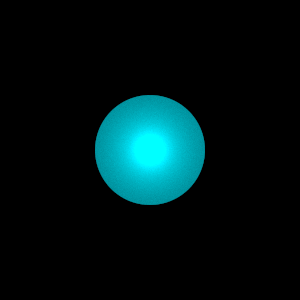
\includegraphics[scale=0.5]{SSL.png}
\caption{Simple Spot Light - light is emitted from 1 point uniformly in cone}
\end{figure}

Fading Spot Light is like Uniform Spot Light, but it is deliberately dimmer further from center of cone.
\begin{figure}[H]
\centering 
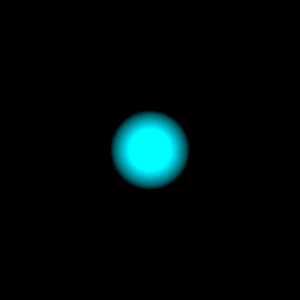
\includegraphics[scale=0.5]{FSL.png}
\caption{Fading Spot Light with slightly higher power}
\end{figure}
To do that, we can create sample set and turn it it into weighted random distribution. Spot light needs (besides position and direction) another parameter - cone angle, which is angle from direction in which beams can be generated. Fading spot light also needs parameter that describes fading. In this example, that parameter is \verb|fade_per_angle|, which describes how much percent dimmer should light shine. From \verb|cone_angle| and \verb|fade_per_adngle|, we can calculate \verb|fade_angle| as (\verb|cone_angle - 1/fade_per_angle|), which is an angle from which onward, light intensity is lowered by value of \verb|fade_per_angle|, per angle. Our Sample set would have $f(x) = 1$ for x from $[0,$\verb|fade_angle|$)$ and $f(x) = 1 - ($\verb|cone_angle| $- x)*$\verb|fade_per_angle| for other. Fading spot light class can look like this:
\begin{lstlisting}[language=Java]
public class  FadingSpotLight extends spdLightSource(){
  private Vector3 perpendicular;
  private WeightedRandomGenerator wrg; 
  private Random circlerot;
 	. . .

  public FadingSpotLight( . . .){
		. . .
	perpendicular = direction.getRandomCross();
	wrg = new WeightedRandomGenerator(. . .);
  }
 . . .
  public Beam getNextBeam(){
	Beam b = new Bean();
	b.lambda = spd.getNextLambda();
	b.origin = position;
	double angle = wrg.nextDouble();
	b.direction = direction.rotateTowards(
	  perpendicular, toRadians(angle));
	angle = circlerot.nextDouble()*360;
	b.direction = b.direction.rotateAround(
	  direction, toRadians(angle)); 
	number_of_beams++;
	return b;
  }
 . . .
}
\end{lstlisting}
\verb|WeightedRandomGenerator wrg| is our weighted random distribution for light intensity which is used to generate angle from [0, \verb|cone_angle|), with increasing bias against bigger angles. Spot light is simetrical on circles(around direction vector), so we can uniformly randomly turn new Beam.direction around spot light direction. This way, fading spot light has adjustable fade towards light cone edge.
\end{document}
